\begin{figure}[ht]
  \centering
  %Define block styles
  \tikzstyle{decision} = [diamond, draw, fill=blue!20, 
  text width=4.5em, text badly centered, node distance=3cm, inner sep=0pt]
  \tikzstyle{block} = [rectangle, draw, fill=blue!20, text width=12em, text
  centered, rounded corners, minimum height=3em]
  \tikzstyle{line} = [draw, -latex']
  \tikzstyle{cloud} = [fill=none, minimum
  height=2em]
  
    
  \begin{tikzpicture}[node distance = 2cm, auto]
    % Place nodes
    \node[cloud] (root) {};
    \node[cloud, left =of root, align=left] (theory) {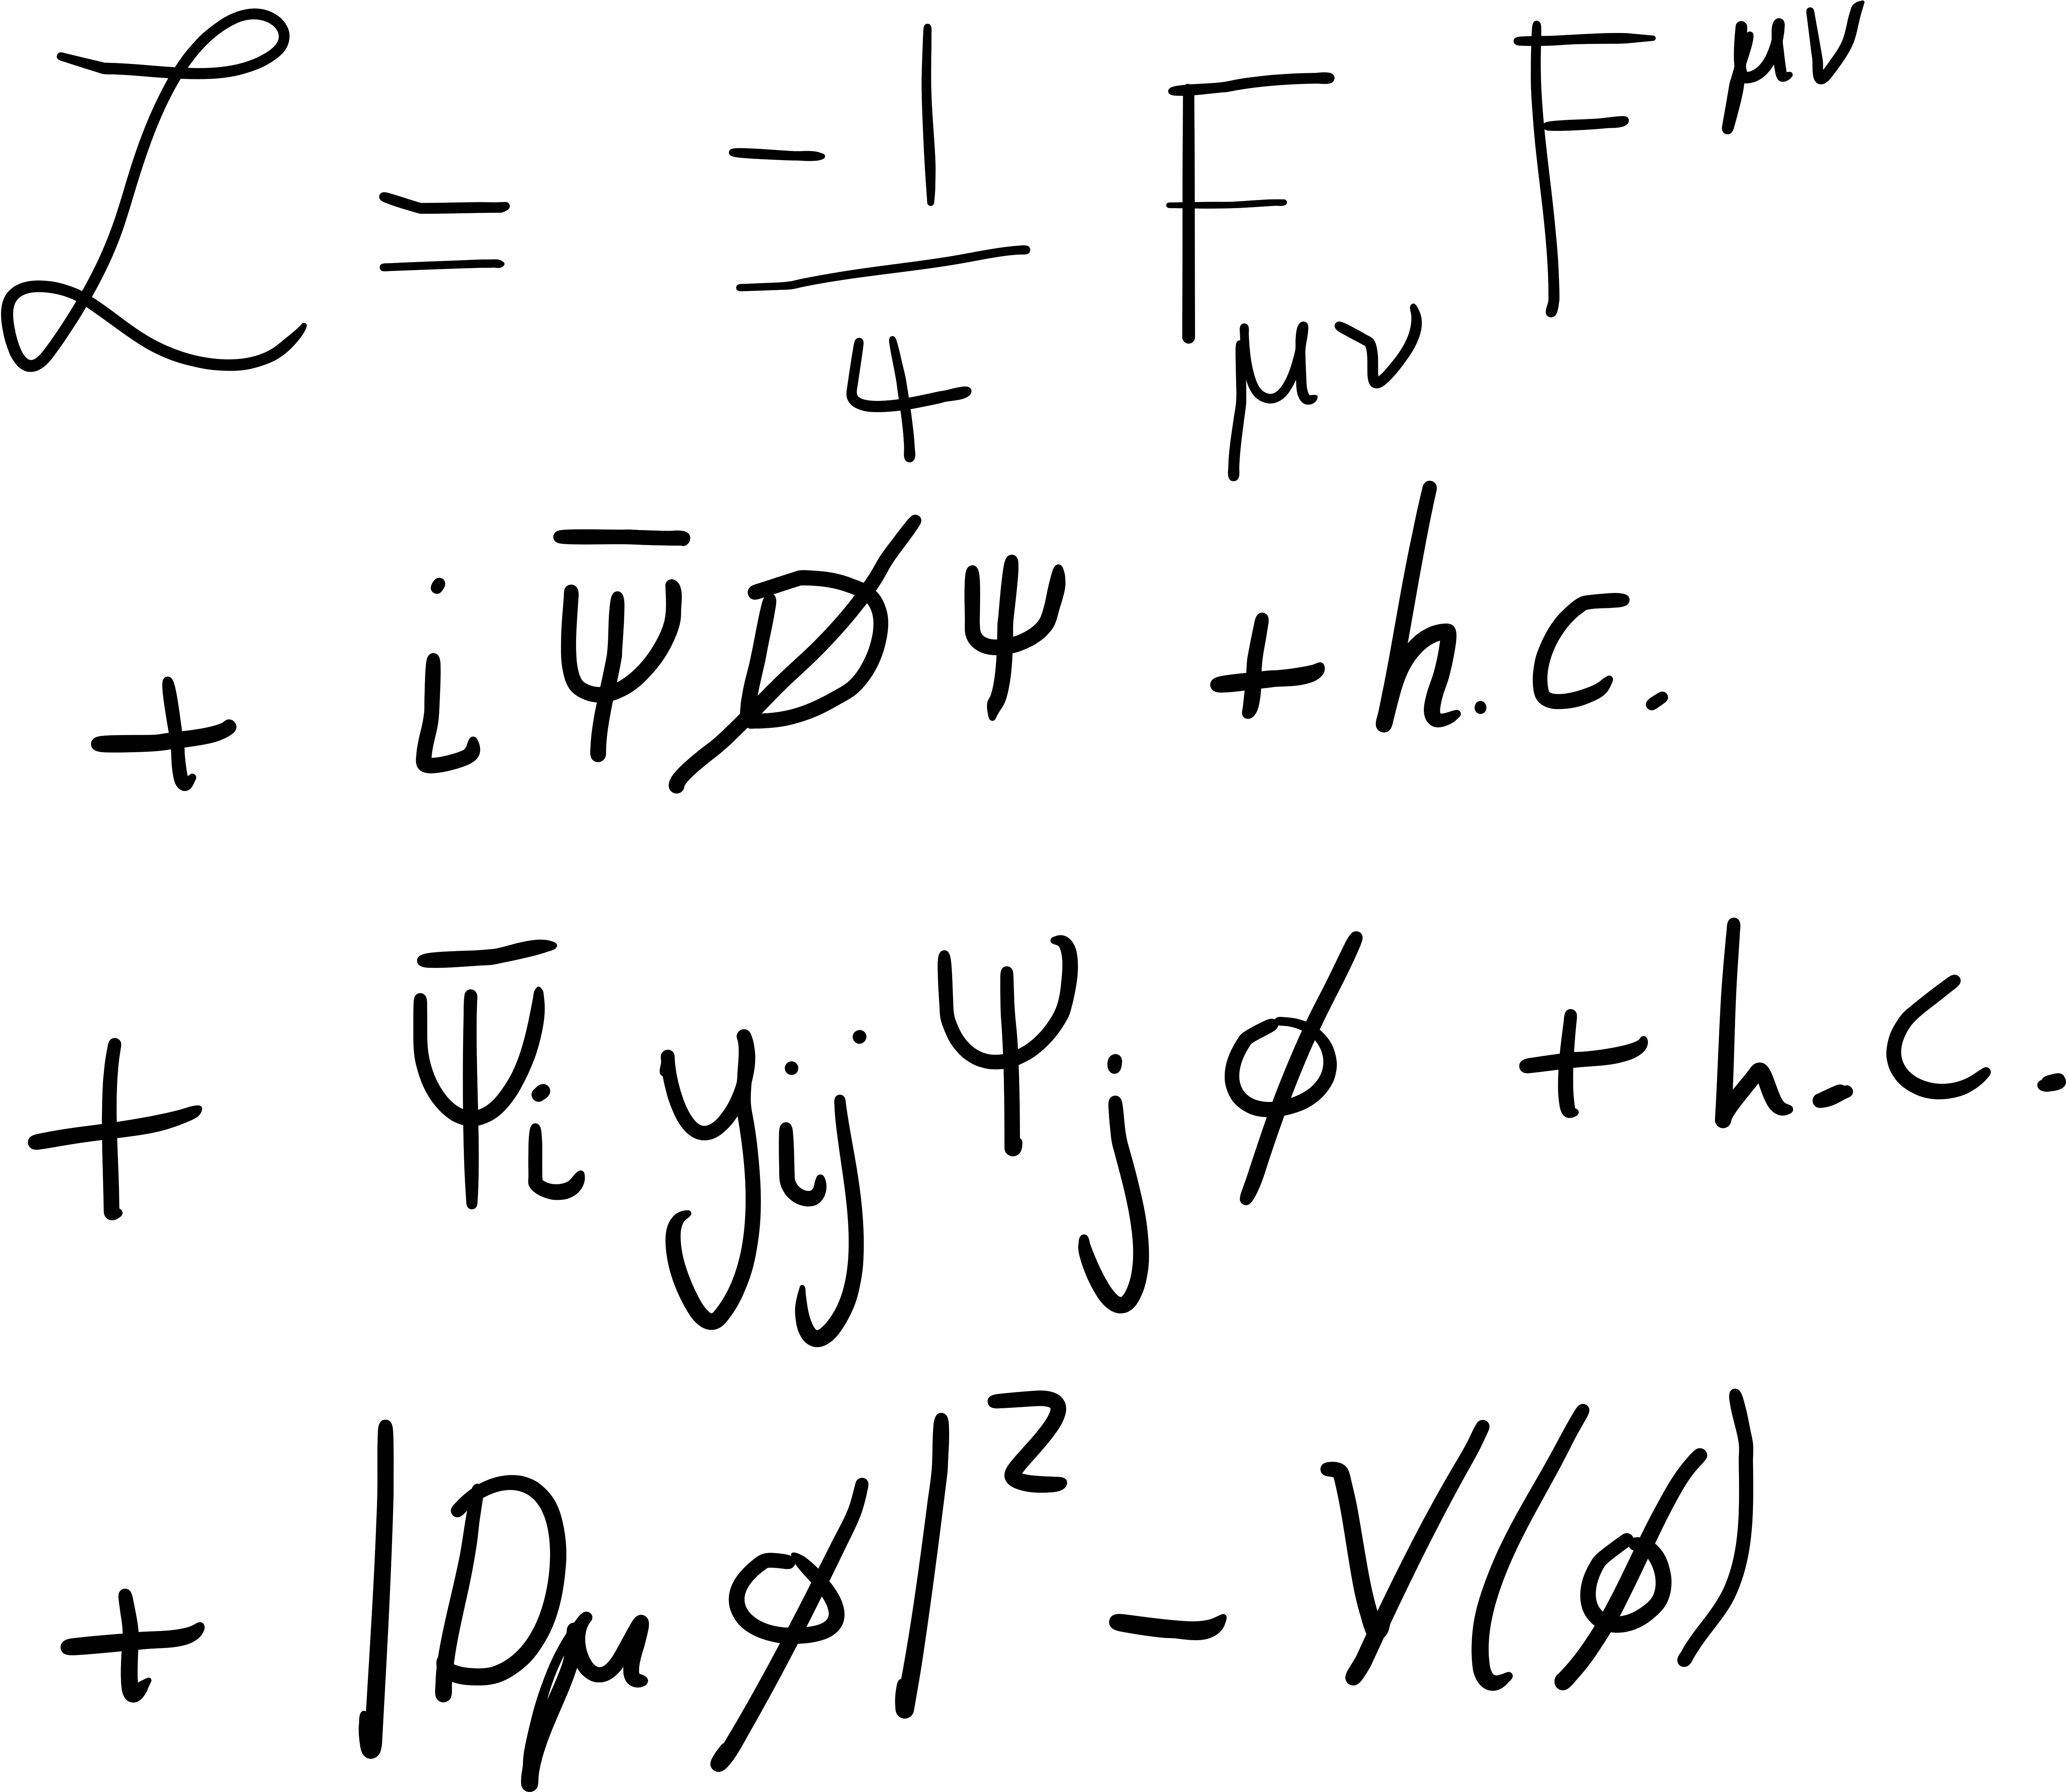
\includegraphics[width=.25\textwidth]{hand_written_lagrangian-1} \\Theory};
    
    \node [cloud, right=of root, align=left] (detector)  {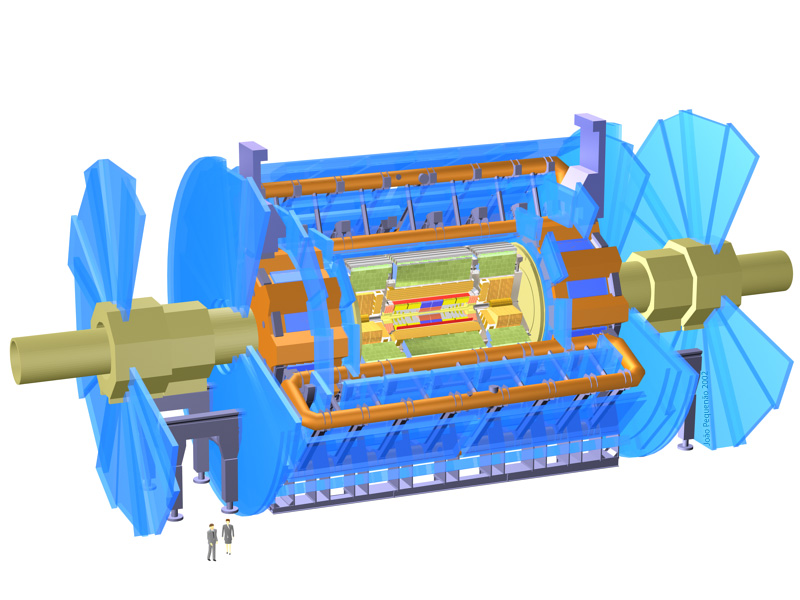
\includegraphics[width=.25\textwidth]{atlas_big} \\Detector};

    \node [cloud, below=of root, align=left] (recon)  {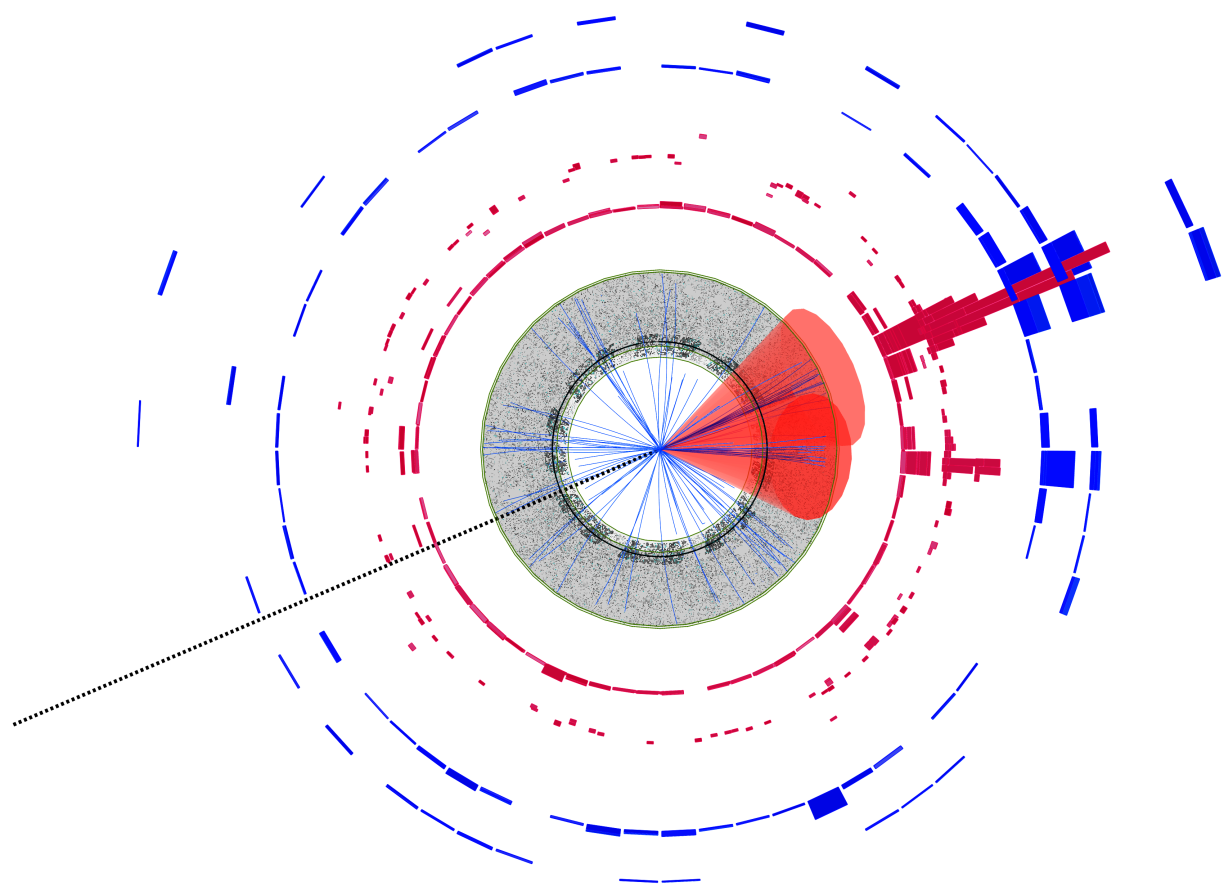
\includegraphics[width=.25\textwidth]{Event_Display_inv} \\Reconstruction};

    \node [cloud, below=of recon] (ghost1) {};
    
    \node [cloud, left=of ghost1, align=left] (modelling)  {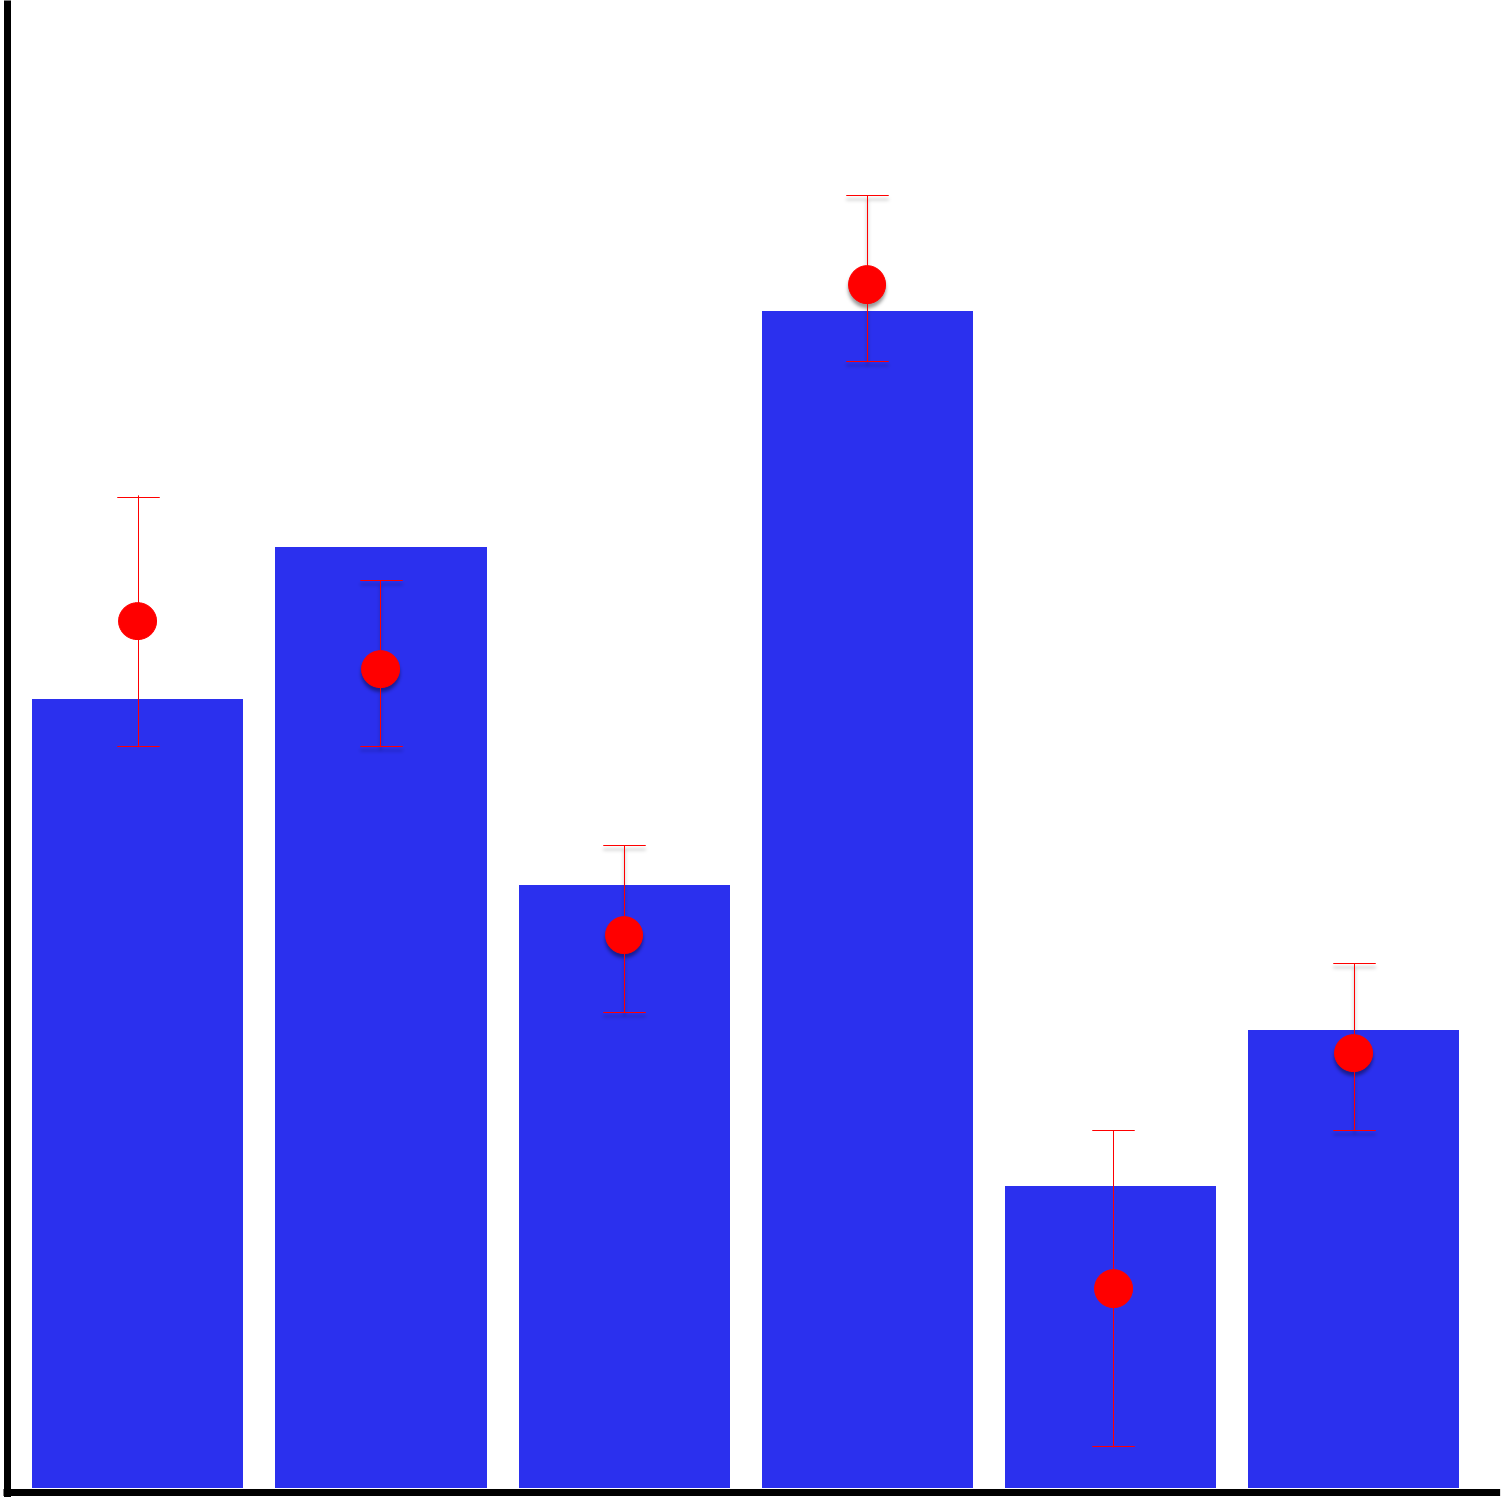
\includegraphics[width=.25\textwidth]{generic_data_mc} \\Modelling};

    \node [cloud, right=of ghost1, align=left] (mva)  {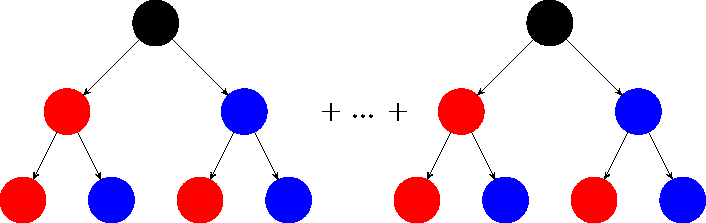
\includegraphics[width=.25\textwidth]{mini-bdt} \\Categorisation};

    \node [cloud, below=of ghost1, align=left] (plf)  {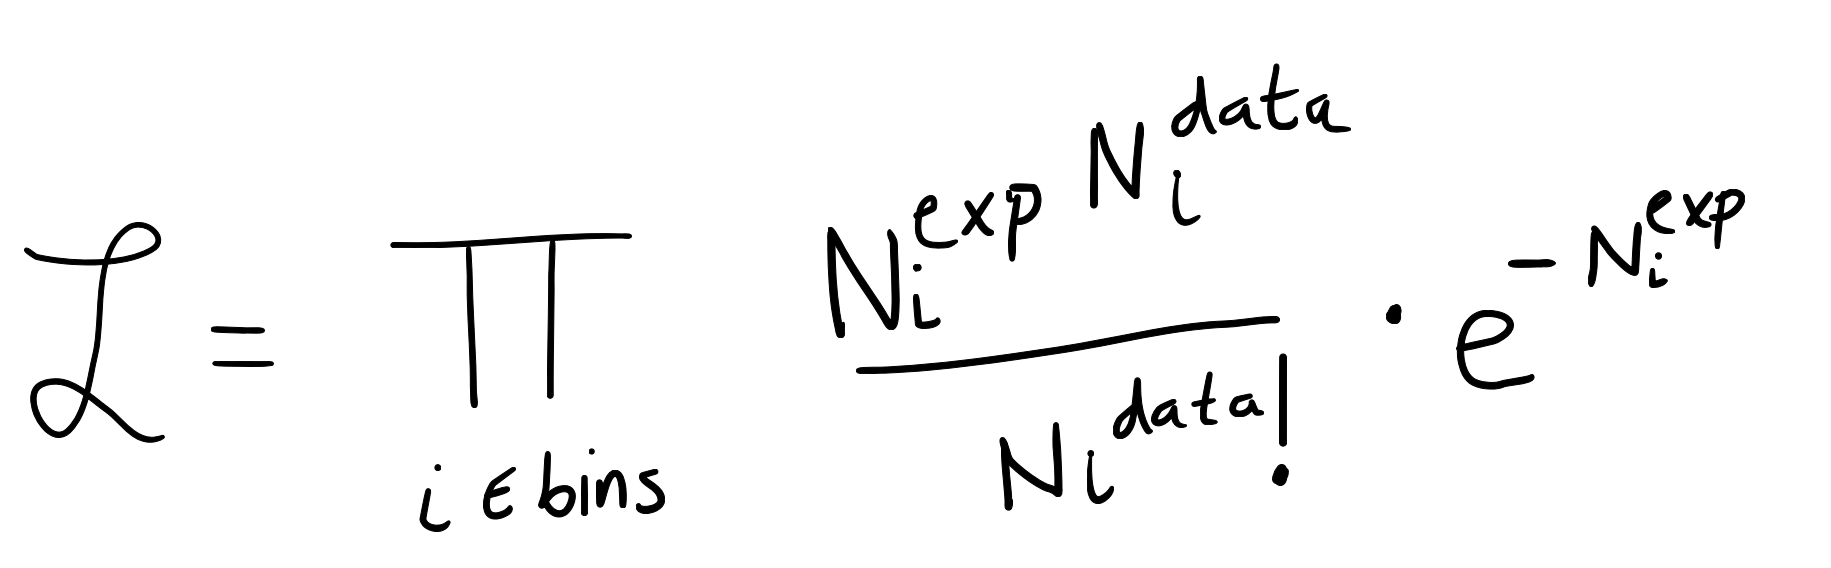
\includegraphics[width=.45\textwidth]{plf_handwritten} \\Profile-Likelihood Fit};

    \node [cloud, below=of plf, align=left] (results)  {
\includegraphics[width=.25\textwidth]{placeholder} \\Results};
    
    % Draw edges 
    \path [line] (theory) -- (detector);

    \path [line] (detector) -- (recon);

    \path [line] (detector) to [out=200,in=70] (modelling);

    \path [line] (recon) -- (modelling);

    \path [line] (recon) -- (mva);

    \path [line] (mva) -- (plf);

    \path [line] (modelling) -- (plf);

    \path [line] (plf) -- (results);
    
  \end{tikzpicture}
  \caption[A roadmap of the analysis.]{A flow chart showing the roadmap of the \VHbb analysis and of this thesis.}
  \label{fig:roadmap}
\end{figure}